\acresetall
\chapter{Introduction}
\label{chap:intro}

\section{Aim and Hypothesis}
Presented in this thesis is my research of which the aim was to build a computational model of the pyloric \ac{CPG} that would accurately reproduce the impact of \ac{DA}, as a neuromodulator, on the neural activity of the \ac{PY} complex. 

Although it has been known for some time that \ac{DA} has a desynchronising effect on the \ac{PY} neurons, no attempts have been made to quantify this effect. The working hypothesis was that the desynchronising impact of \ac{DA} on the \ac{PY} neurons of the \ac{STG} can be quantified such that it is possible to build an accurate computational model of this effect by differentially altering the strength of the gap junctions between the \acp{PY}.

Using electrophysiological and voltage sensitive dye techniques, experiments were devised to capture the effect of \ac{DA} on the \ac{PY} complex. Adequate and appropriate methods to analyse and quantify the captured effects do not seem to be available and thus I suggest new methods for the analysis of \ac{VSD} recordings.

\section{Central Pattern Generators}
\Acp{CPG} are neural circuits that produce rhythmic motor patterns that are involved in actions such as walking, chewing and swimming (See Fig. \ref{fig:cpg_in_walking}). Timing is an inherent function of these circuits and not dependent on sensory or descending inputs \cite{Marder2001}.

\begin{figure}[H]
	\centering 
		\includegraphics[width=5cm]{graphics/cpg_in_walking0.png}
		\caption[Spinal Central Pattern Generators.]{\textbf{Spinal Central Pattern Generators.} \acp{CPG} in the spine that generate rhythmic activity for locomotion without sensory or descending inputs \cite{Lacquaniti1999}}
		\label{fig:cpg_in_walking}
\end{figure}
%See also: http://www.intechopen.com/books/biomechanics-in-applications/mammalian-oral-rhythms-and-motor-control

% 1. Two best known neuro-muscular diseases.
\ac{PDis}\footnote{Parkinson's Disease is usually abbreviated as PD. In research involving the stomatogastric ganglion, however, the abbreviation PD is used for the pyloric constrictor neuron. For the sake of clarity, in the convention adopted for this document, PD is used for the pyloric constrictor neuron and PDis for Parkinson's Disease} and \ac{HD} are probably two of the best known neuromuscular diseases, and are characterised by extremely debilitating impairment of movement. The one thing that these conditions have in common is the destruction of the nerves from the brain that control the \acp{CPG} involved in movement. It is known that \ac{PDis} is caused by the death of dopaminergic neurons; that is, neurons that produce \ac{DA}, which are located in the substantia nigra, a region in the mid-brain \cite{Jankovic2008}. Motor control projections starting from the brain can also be damaged by spinal cord injury or surgery as treatment for conditions such as cancer. % 2. Spinal cord damage

% 3. CPGS are at the core of neuro-muscular control
Walking, running and swallowing are tasks that can be performed without thinking about it. These tasks are made possible by specialised neural networks that are organised in such a way that they can continually repeat particular actions. Known as \acp{CPG}, the circuits produce motor patterns controlling the muscles that allow organisms to produce repetitive movements \cite{Duysens1998, Frigon2011, Marder2005}. The rhythmic patterns produced by \acp{CPG} cannot be explained solely by anatomical connections, but are rather a product of the intrinsic properties \cite{Calabrese1998} of neurons and synaptic interactions. A diversity of patterns is essential for an appropriate response of the network to the changing environments in which organisms find themselves \cite{Selverston1998, Abbott1991}. For optimal performance in changing environmental conditions the patterns need to be adjustable, and this flexibility is provided by sensory and modulatory inputs to the \ac{CPG}.

Although \acp{CPG} can produce rhythms without external input, external inputs allow changes in rhythm for control of, or adaptation to, a changing environment. For instance, it has been found in studies using rats with spinal cord injuries that efficiency in voiding of the bladder is significantly reduced due to disruption of the phasic activity of the external urethral sphincter \cite{Dolber2007}. Treatment with 8-OH-DPAT \footnote{8-OH-DPAT is a chemical that is used to study the function of the 5-HT$_{1A}$ receptor. 5-HT$_{1A}$ is a sub-type of the serotonin (5-HT, 5-hydroxytryptamine) receptor.} \note{Wikipedia: 8-OH-DPAT is a research chemical of the aminotetralin chemical class which was developed in the 1980s and has been widely used to study the function of the 5-HT1A receptor. It was one of the first major 5-HT1A receptor full agonists to be discovered.} showed an increase in micturition volume and a decrease in residual volume resulting from improved voiding efficiency. The improved voiding efficiency can be explained by the induced emergence of phasic external urethral sphincter relaxation. The higher control of the \ac{CPG} that in turn controls the external urethral sphincter is thus severed in spinal cord injury allowing the \ac{CPG} to rhythmically open and close the sphincter much more frequently. The frequent relaxation of the sphincter, in turn, is the cause of the decreased efficiency of voiding of the bladder \cite{Dolber2007}. 


\section{Neuromodulators}
% 4a. The role of neuromodulators
Many diseases are associated with the dysfunction of systems producing neurotransmitters. For example, conditions such as schizophrenia, \ac{PDis} and \ac{ADHD} can, at least in part, be attributed to the body malfunctioning in the production of \ac{DA}. Many systems are affected in very different ways by neuromodulators. Exactly how systems are effected is not always known. Because of the complexity of such systems, research into these diseases is greatly facilitated by the use of model organisms and computational models.

\section{Models}
% 4b. Models are needed
Since it is not always possible to study the causes of diseases or the effect of injuries \textit{in vivo}, we resort to alternatives such as animal model systems, and computational models to find possible causes for a range of conditions and solutions to the problems they produce.

%\note{http://sciencelearn.org.nz/Contexts/The-Noisy-Reef/Science-Ideas-and-Concepts/Scientific-modelling}
A model, in science, is a human construct to help us understand real world systems. Models are used to explain phenomena that cannot be experienced directly. Models can be used to explain complex data, or for generating a hypothesis. Models can also be used for prediction. It is thus very important to select an appropriate type of model for the research at hand.

Animal models are usually selected for their relative tractability compared to that of humans. For instance yeast, \textit{Saccharomyces cerevisiae}, and zebra-fish, \textit{Danio rerio}, are useful for interpreting and understanding the functional and structural mechanisms of human DNA sequences. The genes, the ribosomes and cytoskeletons of \textit{S. cerevisiae} was found to be homologous to that of mammals \cite{Botstein1997, Dooley2000}. Two well-known invertebrates are the fruit fly, \textit{Drosophila melanogaster}, and the nematode worm, \textit{Caenorhabditis elegans}, which serve as model organisms in genetics, genomics and neuroscience. \textit{C. elegans}, for instance, has been favoured as a model organism since the early 1970s due to its experimental amenability, its small well-defined nervous system, the ease with which it can be genetically manipulated and the low cost maintenance \cite{Sengupta2009}.

Computational models are mathematical models of systems such as are found in biology, physics, weather systems etc. Such models can be used to predict the behaviour of these systems in an effort to develop interventions which help to control our environment. By predicting weather systems we can safeguard ourselves against extreme weather conditions or plan our crops to avoid failures. In physics, models serve the purpose of discovering the origins of the universe and predicting what the future might hold for us\note{vague}. In biology, computational models serve to provide a better understanding of the way our bodies work as part of our effort to fight disease and prolong life\note{references}.

The difficulty of building a computational model does not only lie in the creation of the model but also in the selection of parameters and the limitations placed on these parameters to keep the model biologically plausible.

% 5. Models at different scale
Models are built at various scales. There are models that are less detailed with regards to individual neurons but simulate whole areas of the brain. The Blue Brain Project\footnote{\url{http://bluebrain.epfl.ch/}}, for instance, aims to reconstruct the human brain, piece by piece, using a supercomputer to build a virtual brain. The project has already succeeded in simulating a rat cortical column. Such a cortical column has in the range of 10000 neurons and there are about 10000 columns in the cortex of the rat brain. A model such as this, however, simulates each of the neurons in less detail, due to the extensive computing resources required.

There are very detailed models of individual neurons, such as the model created by Hodgkin and Huxley that gives a detailed explanation of how \note{ explain what action potentials are} action potentials are generated and propagated \cite{Hodgkin1952a}. An action potential, sometimes referred to as a spike, is a transient reversal in polarity of the transmembrane potential in a neuron \cite{Barnett2007}. The original Hodgkin-Huxley model is a single compartment model with provision for the three main ion channels responsible for the currents that result in action potentials. This model, however, is easily extendible into multiple compartments and as many ion channels, gap junctions and synapses as are required by the system being modelled. Some of the main problems with detailed models \note{such as Hodgkin-Huxley models???} are computing requirements, the task of finding appropriate solvers for the differential equations used and, perhaps the biggest issue, finding the right parameters for the model.% say something why HH-style conductance based models are good in particular (e.g. they capture more realistic detail than larger scale models)

%6 modelling the STG
The large ganglion in the \ac{STNS} of decapod crustaceans, the \ac{STG} has proved to be an ideal system for studying the effect and impact of neurotransmitters on the generation and variation of rhythmic motor patterns produced by \acp{CPG}. This ganglion consists of about thirty neurons and form two \acp{CPG}, namely the pyloric and the gastric mill \acp{CPG}. These \acp{CPG} control muscles involved in chewing and filtering of food by producing rhythmic patterns. The \ac{STG} is well studied, and the complete connectome of all the neurons in the ganglion is known. The \ac{STG} system is not only ideal for biological research but also for the verification of computational models \cite{Harris-Warrick1992, Selverston2008}. 

Several detailed computer models of \ac{STG} sub-circuits involving a few neurons have been created \cite{Soto-Trevino2005, Golowasch1999a} - we note that these models often simulate multiple neurons of the same kind by a single model neuron (e.g. \ac{PY} or \ac{PD} neurons). Some of the models have been able to show what the effect of neuromodulators on individual neurons and the pyloric rhythm is. These models are still scaled down and model the two \acp{PD} and four to eight \acp{PY} as one \ac{PD} and one \ac{PY}. It is thus not possible to see, from the existing models, what the effect of \ac{DA} would be on the individual \ac{PD}s and \ac{PY}s.

\begin{figure}[H]
	\centering
		\includegraphics[]{graphics/stg_vsd.png}
		\caption[The crab stomatogastric ganglion.]{\textbf{The crab stomatogastric ganglion.} The circular objects are the somas of the neurons. The neurons are arranged around the neuropil which is a collection of axons projecting from the somas.} 
		\label{fig:STG1}
\end{figure}

The objectives of this research were:

\begin{itemize}
	\item To investigate the role of neuromodulation in the regulation of \ac{CPG} activity, using \ac{DA}.
	\item To create a detailed computational model of the pyloric \ac{CPG} capable of showing de-synchronisation of the \ac{PY} complex, that includes the two individual \ac{PD}s, five \ac{PY}s, the lateral pyloric neuron and the \ac{AB}, which in conjunction with the \ac{PD}s serves as a pacemaker group for the pyloric \ac{CPG}.
	\item To accurately model the effect of \ac{DA} on the \acp{PY} in the \ac{STG} of \species{Cancer pagurus}.
	\item To develop numerical methods to quantify measured changes when using electrophysiology and \acp{VSD} such that the output of the biological system can be compared with the output of the computational model.
	\item To investigate alternative methods of simultaneously recording from multiple neurons with the aim of getting better insight into the changes and contributions of individual neurons to the pyloric rhythm under neuromodulatory conditions. These alternative methods are considered for use in conjunction with, or in the place of existing electrophysiological and \ac{VSD} methods currently used on the \ac{STG} to improve quantification of neural behaviour for implementation in computational models.
\end{itemize}

\section{Research Approach}
Using existing models based on the Hodgkin-Huxley equations, a model was developed to include five \ac{PY} neurons, two \ac{PD} neurons, an \ac{AB} neuron and a \ac{LP} neuron. Each neuron was modelled with two compartments. One compartment represents the soma, primary neurite and dendrites and a second compartment represents the axon. All axons were modelled with three currents, $I_{Kd}$, a delayed rectifier current, $I_{Na}$, a fast sodium current and $I_{L}$ a leak current. Parameters for the model were selected from the literature.

In conjunction with the development of the model, electrophysiological recordings and voltage sensitive dye imaging were done on the dissected \ac{STNS} of brown crabs (\textit{Cancer pagurus}). The experiments were designed to provide recordings of the system before, during and after neuromodulation with \ac{DA}.

All methods of recording have some shortcomings. For instance, when using micro-electrodes the number of simultaneously recorded neurons is limited by the physical size of the micro-manipulators. It could also take quite a while to locate the appropriate neurons that is required for an experiment. Neurons are not always located in the same place and therefore, the neurons have to be impaled and recorded from, one by one, until the right one is found. During this process there is always a risk of damaging neuronal cell membranes \cite{Staedele2012}. The use of intra-cellular recording using \ac{VSD} carries the same risk and can be overcome by the use of bath-applied \ac{VSD}. The main drawbacks of all \acp{VSD} are low responsivity, signal to noise ration and toxicity. 

We thus investigated alternative methods that can be used on their own or in conjunction with existing methods, for recording neural activity. The methods investigated are:

\begin{itemize}
	\item Newly developed voltage sensitive dyes
	\item The use of multi-electrode arrays on the \ac{STG}
	\item Injection of dyes using compressed air.
\end{itemize}

The structure of this thesis is as follows. Chapter \ref{chap:background} provides background knowledge of central pattern generators, neuromodulation, existing models and modelling techniques. Chapter \ref{chap:methodsAndMaterials} provides a brief description of the general methods and materials used in the crab laboratory. Chapter \ref{chap:analysis} introduces the methods we developed for the analysis of \ac{VSD} recordings. Following this, we discuss the computational model in chapter \ref{chap:modelling}. 

Two newly developed \acp{VSD}, existing \acp{MEA} recording devices and compressed air injection are methods that have not previously been used on the \ac{STG}. In chapter \ref{chap:alternative} the possibility of successfully using these alternative methods for recording from multiple neurons in the \ac{STG} at the same time are discussed. 


Finally our conclusions and perspectives are presented in chapter \ref{chap:conclusions_perspectives}. 

The \matlab source code of the model can be downloaded from \url{http://www.jannetta.com/downloads/PYCPG_model.zip}



